% Caption for the supplied figures/figure_1.png (unchanged image). Place as figure* at \linewidth: the in-image text is small.
\begin{figure*}[t]
  \centering
  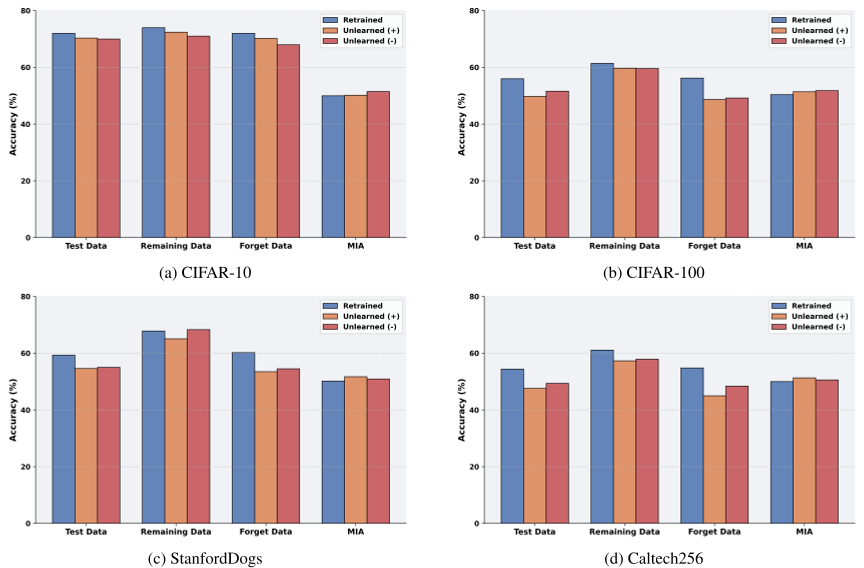
\includegraphics[width=\linewidth]{figures/figure_1.png}
  \caption{Accuracy (\%) on test, remaining and forget data, and MIA score (\%), for Retrained, Unlearned($+$) (exact retain Hessian, needs the source data) and Unlearned($-$) (source-free), in this order from left to right within each group, when 10\% of the training data is forgotten, on (a) CIFAR-10, (b) CIFAR-100, (c) StanfordDogs and (d) Caltech256. Unlearned($-$) stays close to Unlearned($+$) in every panel, and MIA scores of all three models are close to 50\%. On CIFAR-10 the accuracies of Unlearned($-$) are within 4 points of Retrained (\cref{tab:baselines}); in (b)--(d) both unlearned models are a few points below Retrained in accuracy (about 2--7 points, estimated by eye from the bars). Only panel (a) has logged numerical values. No variability estimates are available.}
  \label{fig:main_datasets}
\end{figure*}
